% =====================================================
% Section 2: Methodology
% =====================================================

\section{Methodology}
\label{sec:method}

\begin{figure*}[t]
   \centering
   
    \begin{minipage}[b]{0.75\linewidth}
        \centering
        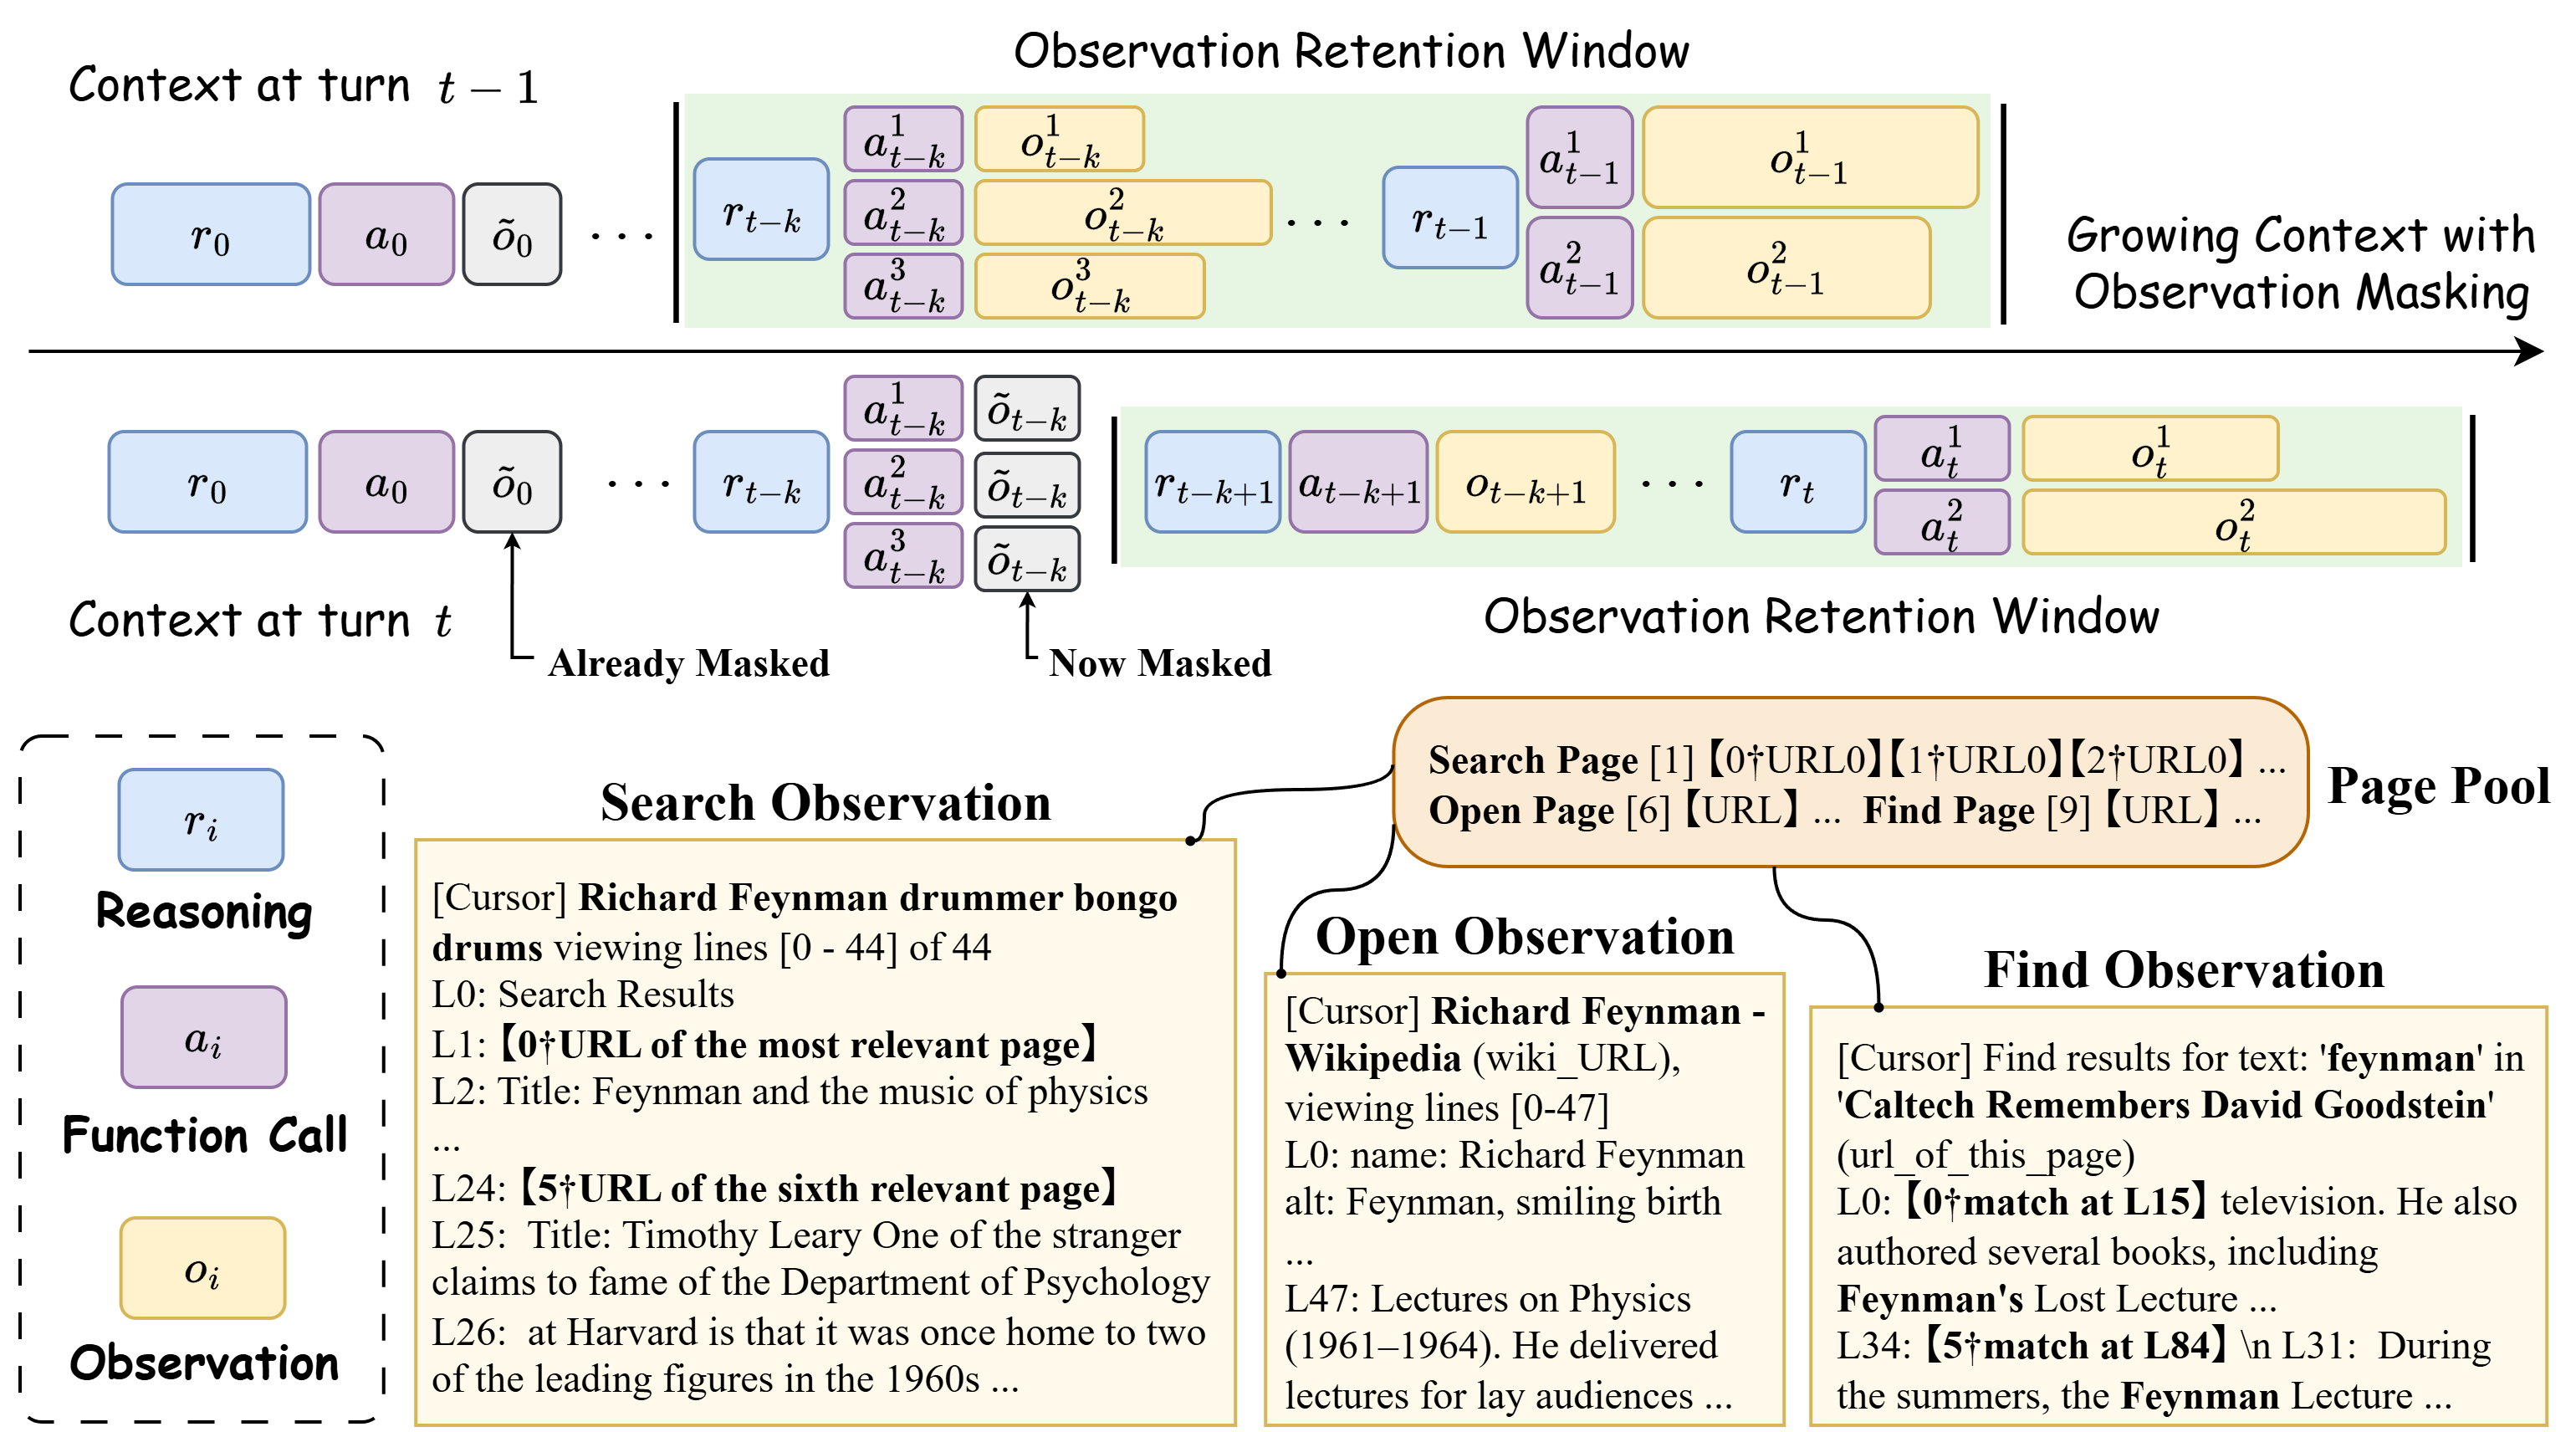
\includegraphics[width=\linewidth]{fig/cm-fig1.png}
        \label{fig1:masking}
    \end{minipage}
    \begin{minipage}[b]{0.24\linewidth}
        \raisebox{-0.5em}{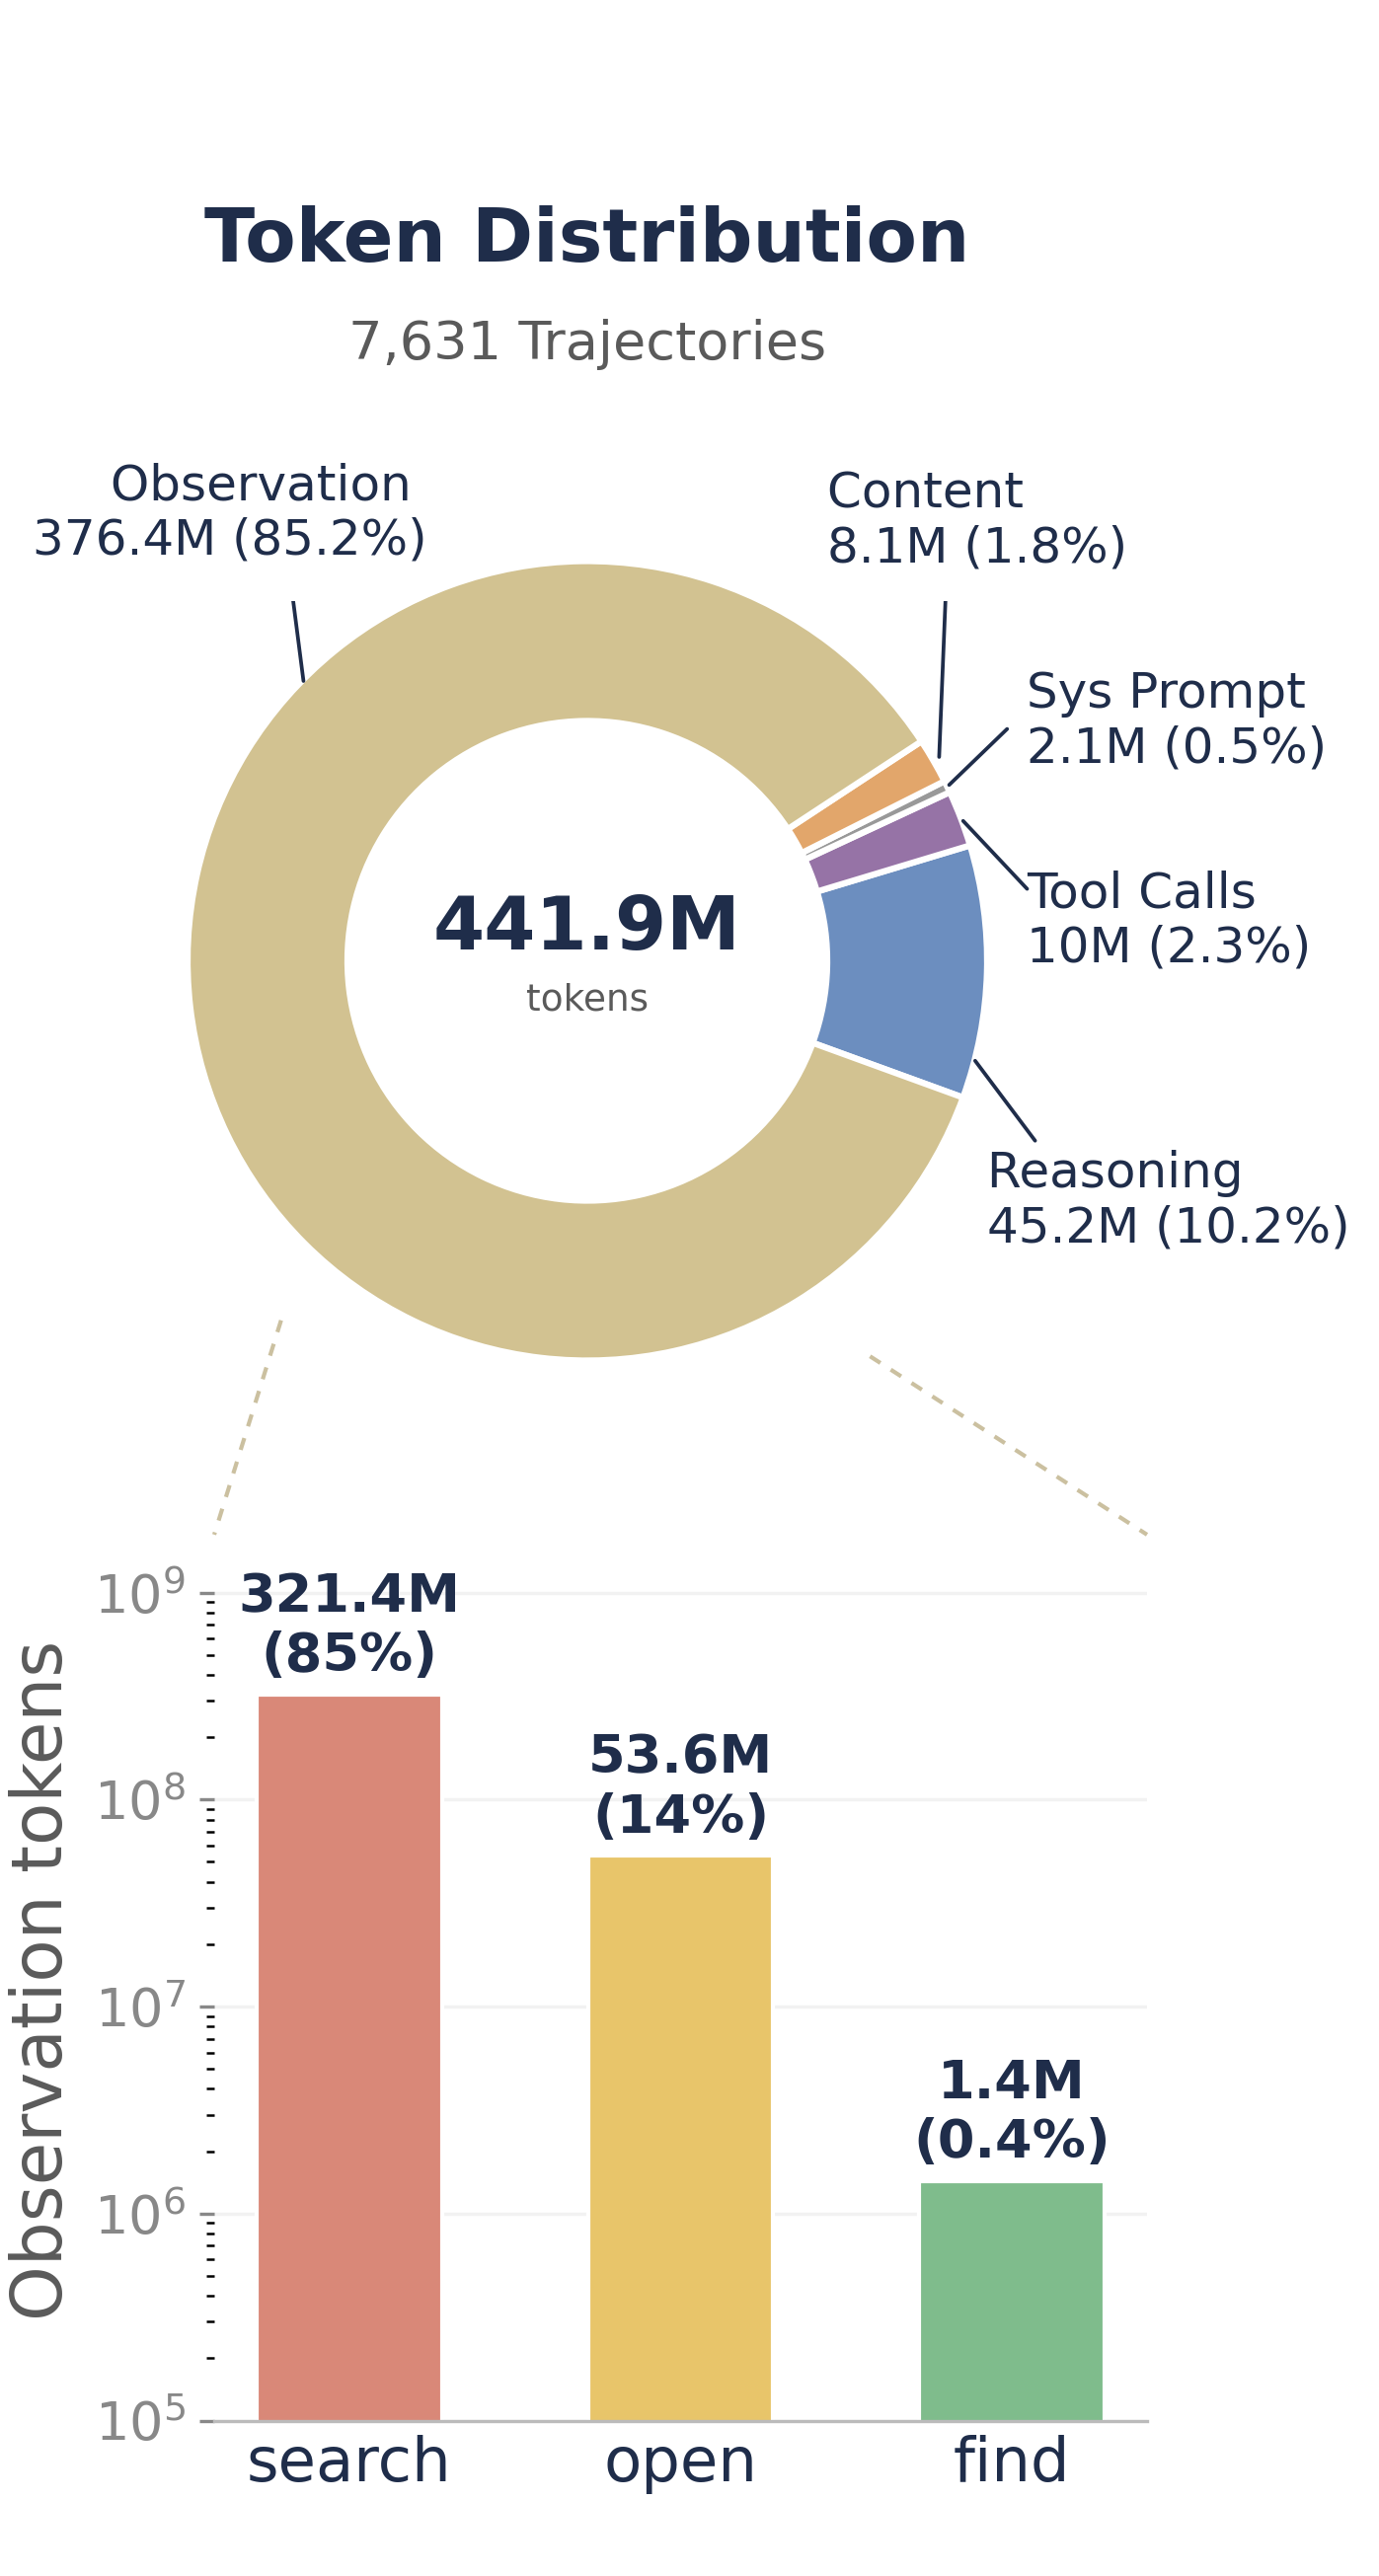
\includegraphics[width=\linewidth]{fig/token-dist-3.png}}
        \label{fig1:pie}
    \end{minipage}
    \vspace{-2.75em}
    \caption{\textbf{Left:} Observation masking at turn $t$. The most recent $K$ observations are retained in the visible context; earlier observations are replaced with a placeholder $\tilde{o}$. Reasoning chains $r_i$, and tool calls $\mathbf{a}_i$ are never masked. Crucially, masking only removes an observation from the model's context. The underlying page remains in the page pool (\S\ref{sec:scaffold}) and stays reachable by its cursor, id, or URL, so the agent can re-open it even after $\tilde{o}$ replaces the original content. \textbf{Right:} Context composition averaged across the Qwen3.5/3.6 family (4B--35B) and three retrievers (BM25, Qwen3-Emb -8B, AgentIR-4B) on BrowseComp-Plus trajectories at termination. Environment observations $\mathbf{o}_i$ account for over 85\% of the overall content tokens, making them the natural target of compression. }
    % \vspace{-1em}
    \label{fig1:pie_main}
\end{figure*}

\subsection{Preliminary}
\label{sec:prelim}

\paragraph{Trajectory.}
A search agent interacts with an environment $\mathcal{E}$ over multiple turns. Given a query $q$, a system prompt $s_0$, and tool metadata $\mathcal{T}_{\text{meta}}$, the agent produces a trajectory $\mathcal{H}_T$ consisting of reasoning--action--observation triplets:
%
\begin{equation}
\label{eq:trajectory}
\mathcal{H}_T = \big\{(q, s_0, \mathcal{T}_{\text{meta}}),\, (r_1, \mathbf{a}_1, \mathbf{o}_1),\, \ldots,\, (r_T, \mathbf{a}_T, o_{T})\big\},
\end{equation}
%
where $r_i$ is the reasoning chain at turn $i$, $\mathbf{a}_i = (a_i^{(1)}, \ldots, a_i^{(k_i)})$ is a set of $k_i \geq 1$ tool calls issued \emph{in parallel}, and $\mathbf{o}_i = (o_i^{(1)}, \ldots, o_i^{(k_i)})$ is the corresponding set of environment observations returned by $\mathcal{E}$. The final action $\mathbf{a}_T$ contains the answer.

\paragraph{Context.}
The agent's policy $\pi$ generates the next reasoning and action conditioned on a \emph{context} $C_t$, which is the linearized trajectory up to turn $t$:
%
\begin{equation}
\label{eq:policy}
(r_t, \mathbf{a}_t) \sim \pi(\,\cdot \mid C_{t-1}),
\ 
C_{t-1} = \textsc{Render}(\mathcal{H}_{t-1}).
\end{equation}
%
The environment then executes $\mathbf{a}_t$ and returns $\mathbf{o}_t = \mathcal{E}(\mathbf{a}_t)$, extending the trajectory as $\mathcal{H}_t = \mathcal{H}_{t-1} \cup \{(r_t, \mathbf{a}_t, \mathbf{o}_t)\}$. The context is then rendered under the selected context management strategy as $C_t = \textsc{Render}(\mathcal{H}_t)$. In long-horizon search, $|C_t|$ grows linearly in $t$ and is dominated by observation tokens $\sum_i |\mathbf{o}_i|$, accounting for the majority of the final context (Figure~\ref{fig1:pie_main}, Right).


\subsection{Observation Masking}
\label{sec:masking}

\paragraph{Stale observations.}
True semantic staleness is latent: an old observation may later become useful if the agent changes its plan.
We therefore use \emph{stale observation} operationally to mean an observation that falls outside a turn-based retention window and is therefore eligible for masking.
This terminology does not assert that the observation is irrelevant.
Rather, it encodes the heuristic that observations usually serve their immediate purpose of informing the next reasoning and action step, and are not often re-read later.
We test this assumption empirically in \S\ref{exp:why}.

\paragraph{Masking.}
Observation masking replaces a stale observation with a fixed \emph{placeholder} $\tilde{o}$, yielding a modified context
%
\begin{equation}
\label{eq:mask}
\widehat{C}_t = \textsc{Render}\!\left(\big\{(r_i, \mathbf{a}_i, m_i(\mathbf{o}_i))\big\}_{i \leq t}\right),
\end{equation}
%
where the masking function $m_i$ retains the $K$ most recent observations but exempts tool-call errors (e.g., malformed arguments, network failures) to allow adaptive debugging:
%
\begin{equation}
\label{eq:mask-fn}
m_i(\mathbf{o}_i) =
\begin{cases}
\mathbf{o}_i & \text{if } \mathbf{o}_i \text{ contains an error}, \\
\mathbf{o}_i & \text{if } i \geq t - K, \\
\tilde{o} & \text{otherwise}.
\end{cases}
\end{equation}
%
Here $K$ is the \emph{retention window}. The placeholder $\tilde{o}$ retains structural information (i.e., which tool was called and with what arguments) but discards the observation content.

\paragraph{Why this formulation.}
Masking is the minimal possible intervention. It neither adds tokens nor requires additional model calls. This minimality is deliberate: we use masking as a \emph{diagnostic instrument} for studying when stale-observation content matters to agent performance, not as a method to be benchmarked against more sophisticated context management techniques.

% =====================================================
% Section 2-2: Scaffold
% =====================================================

\subsection{Scaffold}
\label{sec:scaffold}

Our scaffold is inspired by the rendering conventions of the Harmony format used in~\citep{agarwal2025gptoss}, but formalizes a decoupled, high-concurrency architecture engineered for long-horizon search. Instead of forcing the model to manage raw page content within its volatile context window, our design externalizes environment state into a persistent state object (the \emph{page pool}), provides factored tools to grainily operate over it, and enables parallel tool execution to maximize efficiency per turn. This engineering framework establishes the baseline for subsequent CM analysis.

\paragraph{Page pool.}
Alongside the trajectory $\mathcal{H}_t$ and the context $C_t$ introduced in \S\ref{sec:prelim}, our scaffold maintains a third state object: the \emph{page pool} $\mathcal{P}_t$. It is an append-only sequence of records, where each entry is indexed by a unique, stable cursor $c \in \mathbb{N}$ and stores the page's absolute URL along with its text content. Starting from $\mathcal{P}_0 = \varnothing$, the pool grows monotonically via  $\textsc{NewPages}(\cdot)$ as the agent acts:
\begin{equation}
\label{eq:pool-update}
\mathcal{P}_t \;=\; \mathcal{P}_{t-1} \;\cup\; \textsc{NewPages}(\mathbf{a}_t, \mathbf{o}_t),
\end{equation}
where $\textsc{NewPages}$ deduplicates newly fetched URLs against $\mathcal{P}_{t-1}$. Existing pages retain their original indices, while novel pages are appended with fresh, stable cursors allocated in call order.
Crucially, $\mathcal{P}_t$ is entirely \emph{decoupled} from the volatile context $C_t$. Because pages persist in the pool regardless of whether their corresponding observations are masked out in $\widehat{C}_t$, the agent can seamlessly re-reference any historical page by its cursor without re-issuing an expensive search.

\paragraph{Tools.}
Three tools operate over $(\mathcal{P}_t, \widehat{C}_t)$:

\smallskip
\noindent \underline{\textbf{\texttt{search($q$, topn)}}} issues a retrieval query and returns the top-$\textit{topn}$ snippets. Each snippet is rendered as a self-contained URL link of the form $\text{\cnli} \,\texttt{id} \,\dagger\, \texttt{URL}\,\text{\cnri}$ followed by an abstract.

\smallskip
\noindent \underline{\textbf{\texttt{open(id, cursor, loc, num\_lines)}}} opens a page identified either by a link id from a specified cursor page or by a fully-qualified URL string. The agent may optionally specify a starting line and window size to scope a long page.

\smallskip
\noindent \underline{\textbf{\texttt{find(pattern, cursor)}}} performs exact pattern matching within a page already in $\mathcal{P}_t$ and returns matched line spans, enabling targeted localization without re-reading.

\smallskip
The three tools mirror the canonical agentic-search loop (explore with \texttt{search}, read with \texttt{open}, and localize with \texttt{find}), but factor it so that exploration and reading do not require the agent to regenerate cumbersome URLs.

% \paragraph{Parallel tool calls.}
% To maximize efficiency, each turn $\mathbf{a}_t$ allows $k_t \geq 1$ parallel tool invocations. The page pool processes these concurrently: fresh cursors are allocated in call order, and overlapping results across parallel \texttt{search} actions are deduplicated at the URL level. This concurrency allows the agent to execute multi-perspective exploration in a single turn without inflating the context.

We provide full I/O schemas and context template in Appendix~\S\ref{app:prompts} and \S\ref{app:case-study}, and present a corresponding scaffold ablations in \S\ref{exp:ablation}.